\hypertarget{Fundamentals}{
}

In this chapter, some fundamentals for local illumination models are explained briefly which will be used in the equations and implementation of the reflection models. Since there is a great amount of literature about the mathematical concepts of radiometry and BRDF, these topics are covered only lightly in this chapter. For a more detailed description of these subjects, the reader is advised to look into \cite{RTR} \cite{GlobalIllumination} \cite{DigitalModeling}.

\section{Radiomety}\label{sec:Radiometry}

When dealing with light simulation in the fields of computer graphics or computer vision it is convenient to work with the same quantities as used in the field of optics. The SI unit \footnote[1]{SI unit stands for Système international d'unités, or the International System of Units. It is the most commonly used system in science for system of measurement} for energy of a beam of light is Joules, here denoted by $J$. In physically based rendering we are more interested in the transfer of light over time. The rate of energy transfer per unit time is power, defined as watts in the SI system. Power radiated over a period of time is called radiant flux and expressed as: 

		\begin{eqnarray*}
			\Phi = \Delta J / \Delta t. 
		\end{eqnarray*}

Because the synthesis of images is considered as a momentum in time, the dependency of time is not taken in consideration in further definitions.

The average flux per unit area arriving at the surface is called the irradiance and is defined as the total flux arriving at surface divided by the surface area $A$. Because the surface considered is infinitesimal in area size, the irradiance at an arbitrary point on the surface can be measured by:

		\begin{eqnarray*}
			E = \Phi(x,y) / dA. 
		\end{eqnarray*}

The average flux per unit area leaving the surface is called the radiant exitance and is denoted by $L_o$. The definition is similar to that of the irradiance with the only difference that flux is arriving or leaving the surface. In the field of computer graphics and computer vision, irradiance and radiant exitance are typically denoted by RGB values rather than energy units.

\section{BRDF}

The bi-directional reflectance distribution function (BRDF), first described by {\it Nicodemus et al} \cite{Nicodemus}, can be used as a tool for describing the scattering of light from a surface. This function is assumed to be a local illumination model, meaning that incoming light will be reflected at the point of intersection with the surface \footnote{The BRDF is an approximation of the BSSRDF (Bi-directional scattering surface reflectance distribution function). The BSSRDF simulates the phenomenon of subsurface scattering; light enters the material and after scattering leaves the material at a point different from the intersection point of the incoming light beam.}. Figure \ref{fig:BRDF} shows two cases of light scattering.

The BRDF is a four-dimensional function which is defines the relationship between reflected radiance and irradiance. It is defined in terms of incoming light direction $\omega_i$ and viewing direction $\omega_r$ with respect to the surface normal at a given point on the surface. Both directions are formulated in terms of azimuth angle and zenith angle $\{\theta, \phi\}$. The definition is as follows:

		\begin{eqnarray*}
			f_r(\omega_i, \omega_r) = \frac{dL_o(\omega_r)}{dE(\omega_i)}
		\end{eqnarray*}

\noindent with $dL_o$ the differential outgoing radiance in the viewing direction and $dE$ the differential irradiance. For this research the light sources used are assumed to be point lights (non-area lights at infinite distance), thus simplifying the BRDF to a non-differential form:

		\begin{eqnarray*}
			f_r(\omega_i, \omega_r) = \frac{L_o(\omega_r)}{E_L(\omega_i)\cos \theta_i}
		\end{eqnarray*}

\noindent where $E_L$ is the irradiance of a light source measured on a plane orthogonal to the surface. The cosine term in the denominator is used to calculate the irradiance measured at the surface at a given point and is also known as Lambert's cosine law. With the above equation it is easy to compose a general equation for shading with $n$ non-area lights:

		\begin{eqnarray*}
			L_o(\omega_r) = \sum_{k=1}^n f_r(\omega_{i_k}, \omega_r) \otimes E_{L_k}(\omega_{i_k})\cos\theta_{i_k}
		\end{eqnarray*}

\noindent The $\otimes$ in the equation stands for element-wise multiplication of vectors because the BRDF and the irradiance are both vectors defined in the RGB color space. However, since the synthesis for this research is constraint to grayscale images and the use of one point light, the general equation used in experiments is simplified to:

		\begin{eqnarray*}
			L_o(\omega_r) = f_r(\omega_{i}, \omega_r) \times E_{L}(\omega_{i})\cos\theta_{i}
		\end{eqnarray*}

The BRDF can have many different definitions, resulting in different observed radiant exitance for arbitrary viewpoints. In figure \ref{fig:BRDF}(a) the BRDF has equal radiant exitance in all directions (perfect Lambertian), and in figure \ref{fig:BRDF} a more general BRDF is expressed for diffuse surfaces as the radiant exitance varies for different viewpoints.

\begin{figure}[H]
	\begin{center}
		\subfigure[ ]{
\epsfig{file=images/LambertianReflection.eps, width=0.4\linewidth}}
		\subfigure[ ]{
\epsfig{file=images/GeneralReflection.eps, width=0.4\linewidth}}
	\end{center}
	\caption{{\it Two cases of reflection. (a) shows ideal Lambertian reflection and (b) shows general diffuse reflection.}}
	\label{fig:BRDF}
\end{figure}

\section{Lambert's Cosine Law}

The previous section defines the irradiance in the simplified BRDF and the general shading equation as $E_L$, the irradiance measured in a plane orthogonal to the surface. The cosine term is used to measure the irradiance at a point on the surface. To get a better understanding of this relation, we can inspect the behavior of irradiance at a diffuse surface on microscopic level.

\begin{figure}[H]
	\begin{center}
		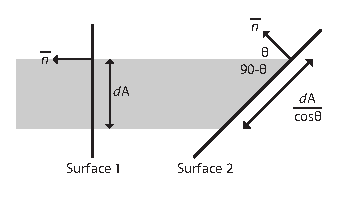
\epsfig{file=images/LambertCosineLaw.eps, width=0.5\linewidth}
	\end{center}
	\caption{{\it The beam shown in gray gets projected on an area $dA$ on both surface 1 and surface 2. The area covered by the beam on surface 1 is $dA$, and on surface 2 is $\frac{dA}{\cos\theta}$. \tit{Image adapted from Computer Graphics, Principles and Practice \cite{ComputerGraphics}}}}
	\label{fig:BEAM}
\end{figure}

If we look at figure \ref{fig:BEAM}, we can see how an incoming light beam with unit energy is projected on an infinitesimal area $dA$ on the surface. If the surface normal and the light direction are parallel and in the same direction as is the case with {\it Surface 1}, the energy received and reflected by the area is proportional to $dA$. If the beam is projected on the surface such that it covers a larger area as is the case with {\it Surface 2}, the amount of energy reflected from area $dA$ is proportional to $\cos \theta$. The amount of energy reflected per unit area is less on {\it Surface 2} compared to {\it Surface 1} since the energy contained by the beam covers a larger area. This observation of radiance behaviour is also known as Lambert's Cosine Law. 


